\documentclass{standalone}
\usepackage[dvipsnames,svgnames,x11names]{xcolor}
\usepackage{tikz}
\usepackage{pgfplots}
\usetikzlibrary{pgfplots.statistics}
\pgfplotsset{compat = 1.12}
\usepackage[
  group-separator={,},
  exponent-product=\cdot,
]{siunitx}
\usepackage{../thesismath}
\begin{document}
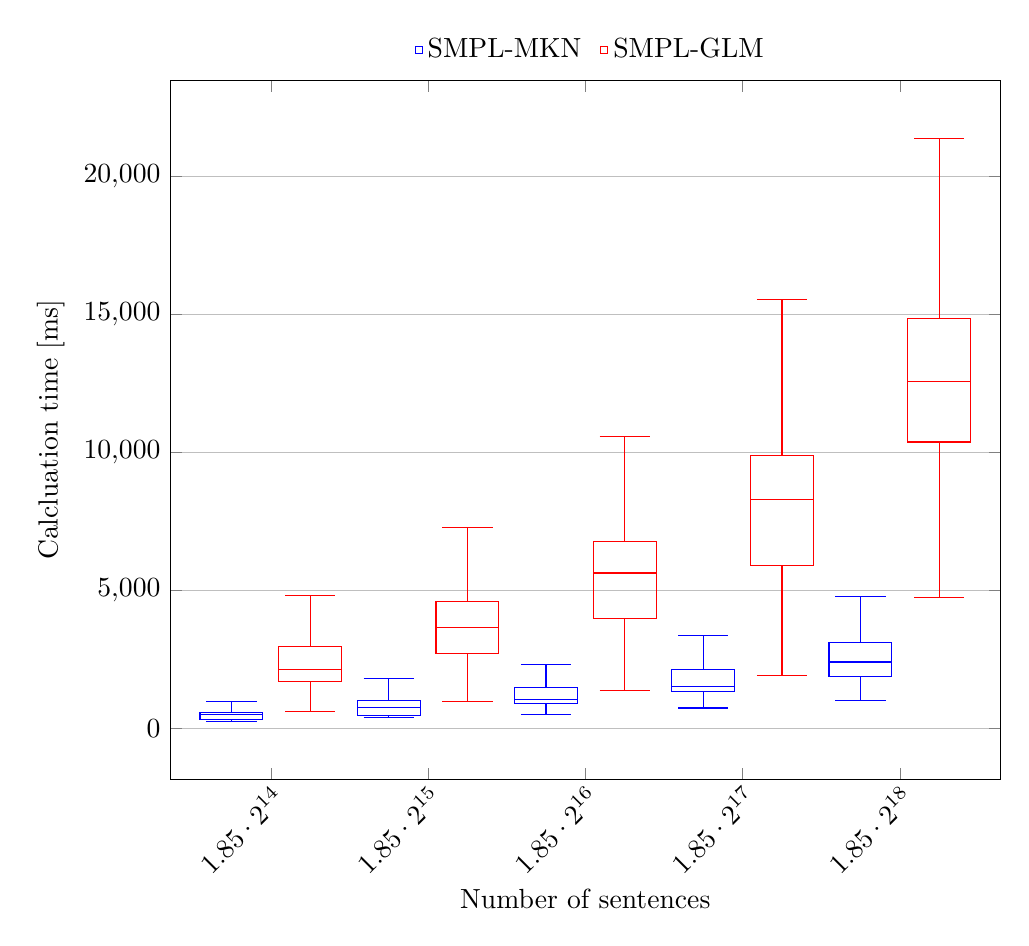
\begin{tikzpicture}[baseline]

\pgfplotscreateplotcyclelist{mkn_glm}{%
  blue,  mark size=1.25, mark=square,\\%
  red,   mark size=1.25, mark=square,\\%
}

\pgfplotsset{
  legend style = {
    draw = none,
    legend image code/.code = {
      \draw[only marks]
        plot coordinates {
          (0.3cm,0cm)
        };
      \node at (0.15cm, 0cm) {};
    },
  },
  boxplot/draw/average/.code = {
    %% uncomment to show dotted bars for average:
    %\draw[dashed, /pgfplots/boxplot/every average/.try]
    %  (boxplot box cs:\pgfplotsboxplotvalue{average},0)
    %  --
    %  (boxplot box cs:\pgfplotsboxplotvalue{average},1)
    %  ;
  },
}

\sisetup{exponent-base = 2}
\begin{axis}[
  xlabel = {Number of sentences},
  xtick       = {            1,             2,             3,             4,             5},
  xticklabels = {\num{1.85e14}, \num{1.85e15}, \num{1.85e16}, \num{1.85e17}, \num{1.85e18}},
  xticklabel style={
    inner sep = 1pt,
    anchor = north east,
    rotate = 45,
  },
  ylabel = {Calcluation time [\si{\milli\second}]},
  scaled y ticks = false,
  log ticks with fixed point,
  boxplot/draw direction = y,
  cycle list name = mkn_glm,
  grid = major,
  xmajorgrids = false,
  legend entries = {{SMPL-MKN}, {SMPL-GLM}},
  legend style = {
    anchor=south,
    at={(axis description cs: 0.5, 1.01)}
  },
  legend columns = 3,
  width = \textwidth,
]

% training-5-argmaxcompare-1k-c/ngram-5-1k-SMPL-Weighted-Sum-Modified-Kneser-Ney-1
\addplot+[
  boxplot prepared = {
    %draw position = 30400,
    draw position = 1,
    box extend = 0.4,
    lower whisker = 265.492867,
    lower quartile = 314.299584,
    median = 502.856222,
    upper quartile = 579.864225,
    upper whisker = 976.748291,
    average = 513.082405,
  },
  xshift = -0.5cm,
] table [row sep = \\, y index = 0] {
  data\\
};

% training-5-argmaxcompare-1k-c/ngram-5-1k-SMPL-Weighted-Sum-Generalized-Language-Model-1
\addplot+[
  boxplot prepared = {
    %draw position = 30400,
    draw position = 1,
    box extend = 0.4,
    lower whisker = 622.720529,
    lower quartile = 1706.427235,
    median = 2121.929949,
    upper quartile = 2958.550537,
    upper whisker = 4831.142348,
    average = 2362.456282,
  },
  xshift = 0.5cm,
] table [row sep = \\, y index = 0] {
  data\\
};

% ------------------------------------------------------------------------------

% training-4-argmaxcompare-1k-c/ngram-5-1k-SMPL-Weighted-Sum-Modified-Kneser-Ney-1
\addplot+[
  boxplot prepared = {
    %draw position = 60801,
    draw position = 2,
    box extend = 0.4,
    lower whisker = 385.966344,
    lower quartile = 473.753359,
    median = 758.676964,
    upper quartile = 1014.005158,
    upper whisker = 1802.043448,
    average = 800.724252,
  },
  xshift = -0.5cm,
] table [row sep = \\, y index = 0] {
  data\\
};

% training-4-argmaxcompare-1k-c/ngram-5-1k-SMPL-Weighted-Sum-Generalized-Language-Model-1
\addplot+[
  boxplot prepared = {
    %draw position = 60801,
    draw position = 2,
    box extend = 0.4,
    lower whisker = 961.789997,
    lower quartile = 2718.921302,
    median = 3658.357928,
    upper quartile = 4589.696867,
    upper whisker = 7276.519473,
    average = 3731.691975,
  },
  xshift = 0.5cm,
] table [row sep = \\, y index = 0] {
  data\\
};


% ------------------------------------------------------------------------------

% training-3-argmaxcompare-1k-c/ngram-5-1k-SMPL-Weighted-Sum-Modified-Kneser-Ney-1
\addplot+[
  boxplot prepared = {
    %draw position = 121602,
    draw position = 3,
    box extend = 0.4,
    lower whisker = 518.403279,
    lower quartile = 898.427997,
    median = 1050.791946,
    upper quartile = 1476.127982,
    upper whisker = 2317.160040,
    average = 1156.278226,
  },
  xshift = -0.5cm,
] table [row sep = \\, y index = 0] {
  data\\
};

% training-3-argmaxcompare-1k-c/ngram-5-1k-SMPL-Weighted-Sum-Generalized-Language-Model-1
\addplot+[
  boxplot prepared = {
    %draw position = 121602,
    draw position = 3,
    box extend = 0.4,
    lower whisker = 1364.652392,
    lower quartile = 3988.427046,
    median = 5634.106144,
    upper quartile = 6779.049736,
    upper whisker = 10592.623255,
    average = 5539.993735,
  },
  xshift = 0.5cm,
] table [row sep = \\, y index = 0] {
  data\\
};

% ------------------------------------------------------------------------------

% training-2-argmaxcompare-1k-c/ngram-5-1k-SMPL-Weighted-Sum-Modified-Kneser-Ney-1
\addplot+[
  boxplot prepared = {
    %draw position = 2432004,
    draw position = 4,
    box extend = 0.4,
    lower whisker = 739.370986,
    lower quartile = 1335.713467,
    median = 1535.447582,
    upper quartile = 2146.337549,
    upper whisker = 3356.148393,
    average = 1727.968135,
  },
  xshift = -0.5cm,
] table [row sep = \\, y index = 0] {
  data\\
};

% training-2-argmaxcompare-1k-c/ngram-5-1k-SMPL-Weighted-Sum-Generalized-Language-Model-1
\addplot+[
  boxplot prepared = {
    %draw position = 2432004,
    draw position = 4,
    box extend = 0.4,
    lower whisker = 1916.275703,
    lower quartile = 5904.384880,
    median = 8297.770319,
    upper quartile = 9906.363211,
    upper whisker = 15555.723291,
    average = 8229.612393,
  },
  xshift = 0.5cm,
] table [row sep = \\, y index = 0] {
  data\\
};

% ------------------------------------------------------------------------------

% training-1-argmaxcompare-1k-c/ngram-5-1k-SMPL-Weighted-Sum-Modified-Kneser-Ney-1
\addplot+[
  boxplot prepared = {
    %draw position = 486409,
    draw position = 5,
    box extend = 0.4,
    lower whisker = 1002.784867,
    lower quartile = 1886.653179,
    median = 2408.640801,
    upper quartile = 3109.965427,
    upper whisker = 4779.094746,
    average = 2527.778769,
  },
  xshift = -0.5cm,
] table [row sep = \\, y index = 0] {
  data\\
};

% training-1-argmaxcompare-1k-c/ngram-5-1k-SMPL-Weighted-Sum-Generalized-Language-Model-1
\addplot+[
  boxplot prepared = {
    %draw position = 486409,
    draw position = 5,
    box extend = 0.4,
    lower whisker = 4741.025183,
    lower quartile = 10381.878531,
    median = 12565.672071,
    upper quartile = 14875.880460,
    upper whisker = 21379.195192,
    average = 12622.954410,
  },
  xshift = 0.5cm,
] table [row sep = \\, y index = 0] {
  data\\
};

\end{axis}

\end{tikzpicture}
\end{document}
